\subsection{Tempo di propagazione}

\begin{wrapfigure}[10]{l}{0.5\textwidth}
\centering
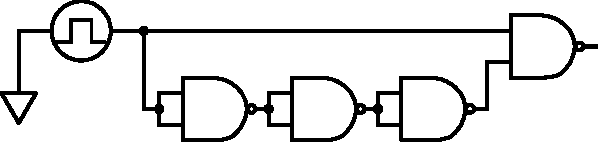
\includegraphics[width=.4\textwidth]{../E10/latex/delay.pdf}
\caption{Schema del circuito utilizzato per misurare il Propagation Delay Time (PDT) di una porta NAND.}
\label{cir10:delay}
\end{wrapfigure}


In questa prima parte dell'esperienza analizzeremo il PDT (Propagation Delay Time) di una porta NAND.
Tale parametro è il ritardo con cui l'uscita commuta rispetto all'istante in cui commuta l'ingresso.
Poichè tale intervallo temporale è di pochi \si{\nano\second}, è stato deciso di collegare in serie 3 porte NOT.
Così facendo il ritardo viene amplificato di 3 volte.
Possiamo ora costruire il circuito riportato in Figura \ref{cir10:delay}.

Come vediamo, se non esistesse il ritardo l'uscita sarebbe sempre ad 1 logico ($\approx 5 \si{\volt}$).
A causa del ritardo, però, quando il segnale in ingresso commuta da 0 ad 1, la serie di porte NOT non riuscità instantaneamente a passare da 1 a 0 e dunque, per un breve intervallo entrambi gli ingressi saranno ad 1 logico il che implica un uscita a 0 logico.
Abbiamo utilizzato in ingresso un'onda quadra ($V_{pp}=\SI{5}{\volt}$, $V_{off}=+\SI{2.5}{\volt}$, $\nu=\SI{100}{\kilo\hertz}$).
Notiamo che la presenza della porta NAND in uscita non da contributo al ritardo totale in quanto essa provoca solo uno shift temporale, non un aumento del delay.
Il valore ch stimeremo dal grafico dovrà dunque essere diviso per 3, in modo da ottenere il tempo di propagazione di una singola porta.

\begin{figure}[htpc]
\centering
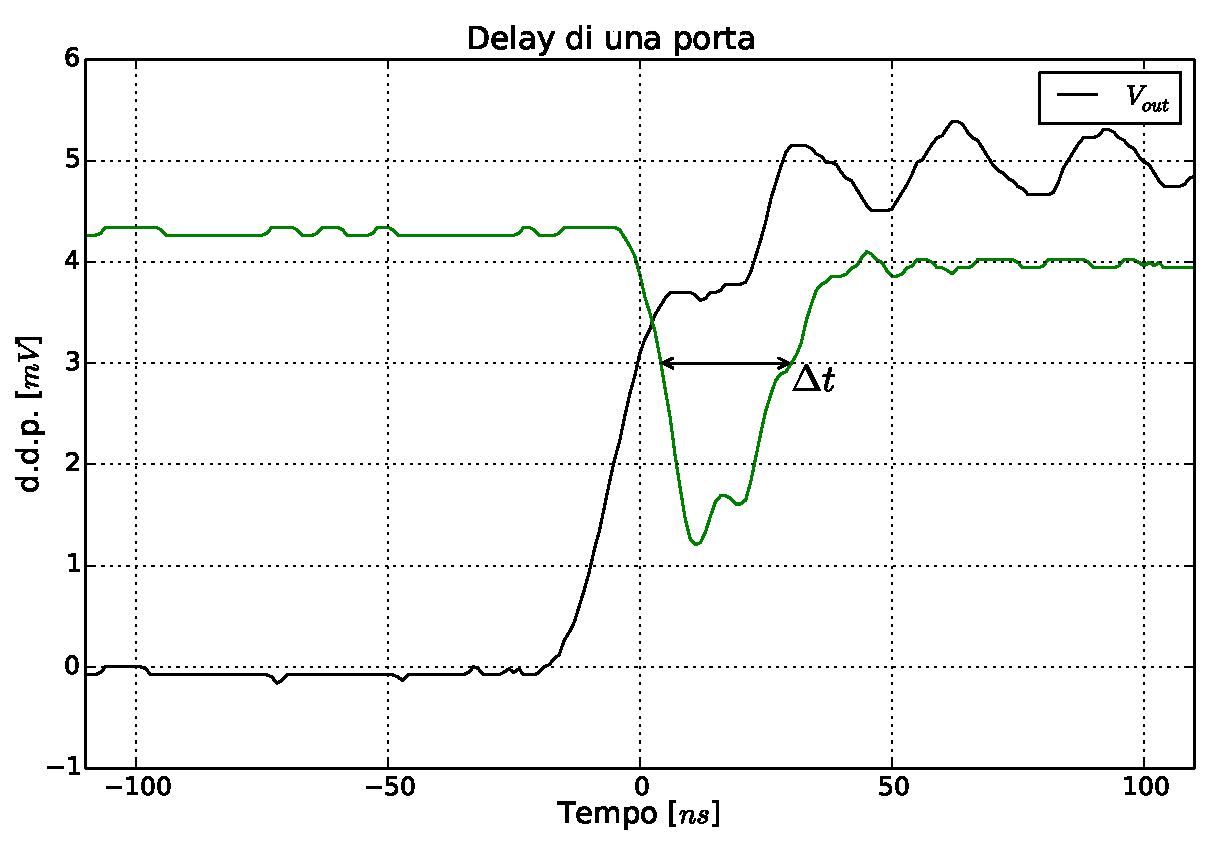
\includegraphics[width=.65\textwidth]{../E10/latex/gdelay.pdf}
\caption{Grafico che mostra la risposta la risposta in uscita del circuito in Figura \ref{cir10:delay} al cambiamento di stato (da 0 a \SI{5}{\V}) dell'onda quadra in ingresso.}
\label{gr10:delay}
\end{figure}

Come vediamo il segnale non è perfettamente un'onda quadra, nè in ingresso nè in uscita.
Ciò è dovuto alle impedenze parassite e alle correnti assorbite dalla porta.
Abbiamo dunque deciso di prendere i valori temporali al 50\% dell'ampiezza massima.
I valori ottenuti sono \SI{26\pm 2}{\nano\second}.
Il valore Per la singola porta è dunque \SI{9\pm 1}{\nano\second}, valore compatibile con i valori riportati sul datasheet.

\subsection{Verifica di una porta NOT TTL Open Collector }

\begin{wrapfigure}[17]{r}{0.3\textwidth}
\centering
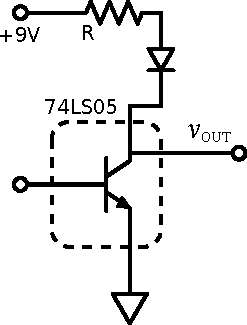
\includegraphics[width=.2\textwidth]{../E10/latex/open_collector.pdf}
\caption{Schema del circuito utilizzato per la verifica di funzionamento di una porta NOT open collector.}
\label{cir10:open_collector}
\end{wrapfigure}

Questa seconda parte dell'esperienza prevede la verifica di una porta NOT TTL Open Collector.
Tali porte sono particolarmente utili quando vogliamo passare tra logiche che lavorano a tensioni diverse.
Infatti, avendo il collettore aperto, possiamo collegare il collettore stesso ad una tensione diversa rispetto a quella con cui è alimentata la porta.
Nel nostro caso, abbiamo utilizzato una porta TTL (0/+5 \si{\volt}) e abbiamo collegato il collettore a +9\si{\volt}.
Per la verifica abbiamo deciso di utilizzare un led luminoso.
Lo schema circuitale è riportato in Figura \ref{cir10:open_collector}.

Considerando una caduta di circa \SI{1.5}{\volt} sul led e una corrente di \SI{5}{\milli\ampere}, e una caduta data dal transistor della porta di circa \SI{0.5}{\volt} possiamo facilmente calcolare, usando la legge di Ohm, la resistenza necessaria.
Il valore scelto alla fine anche per comodità è di \SI{1.5}{\kilo\ohm}.

Ricordiamo che il transistor che compone la nostra porta sarà in saturazione quando la tensione in ingresso è alta, e dunque avremo un'uscita bassa.
Invece, quando all'ingresso avremo uno zero logico, il transistor sarà interdetto e dunque avremo una tensione alta in uscita.


Il circuito è stato verificato infine utilizzando l'oscilloscopio.
I dati sono riportati nel seguente grafico.

\begin{figure}[htpc]
\centering
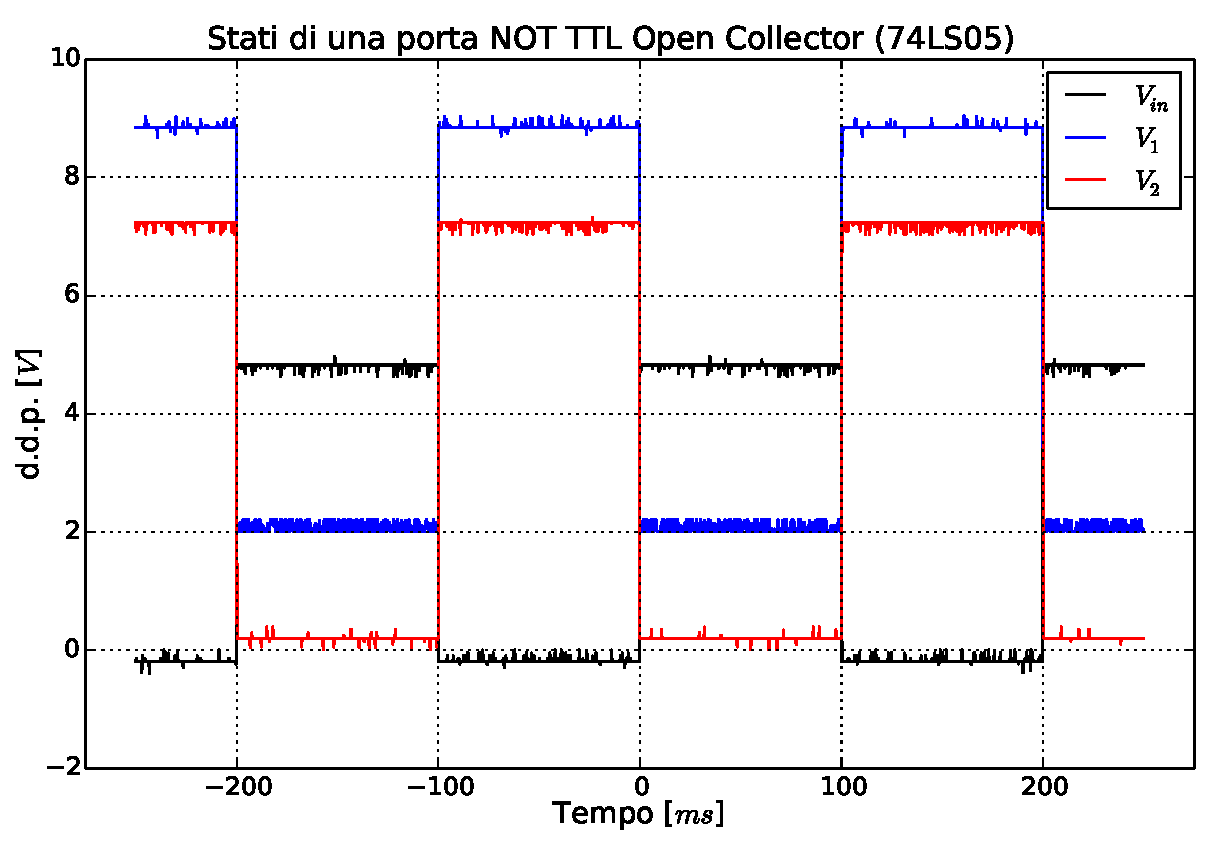
\includegraphics[width=.65\textwidth]{../E10/latex/NOTTTL.pdf}
\caption{Grafico che mostra l'onda in entrata e la risposta del circuito presa in due punti differenti: $V_1$ è stata misurata tra la resistenza $R$ e il diodo, mentre $V_2$ è stata misurata tra il diodo e l'uscita della porta NOT.}
\label{gr10:notttl}
\end{figure}

Come vediamo dal grafico, la tensione di 0 logico è circa \SI{0.4}{\volt}, valore coerente con quello atteso data la caduta della giungione base-emettitore del transistor.
Tuttavia, se preleviamo la tensione in uscita sotto il diodo, abbiamo come tensione alta \SI{7.4}{\V}.
Ciò non è aspettato in quanto dovremmo trovare la stessa tensione di alimentazione (+\SI{9}{\V}).
Abbiamo allora provato a prelevare la tensione sopra il diodo, ottendendo una tensione alta di \SI{9}{\V} ed una bassa di \SI{2}{\V}.
Tale valore, ovviamente, è dovuto al fatto che abbiamo una caduta sia sul diodo ($\approx \SI{1.5}{\V}$) sia sul transistor ($\approx$ \SI{0.5}{\V}).

Abbiamo provato a misurare, utilizzando l'amperometro, la corrente che scorre nel ramo di collettore.
Il risultato ottenuto è che la corrente è dell'ordine dei \si{\micro\ampere}, cosa aspettata  in quanto il transistor è in interdizione.
Non siamo riusciti a capire perchè il diodo provocasse una caduta in tensione di $\approx \SI{1.5}{\volt}$ anche quando attraverso esso non scorreva corrente.

\newpage
\subsection{Verifica di una porta buffer TTL 3State}

\begin{wrapfigure}[14]{l}{0.5\textwidth}
\centering
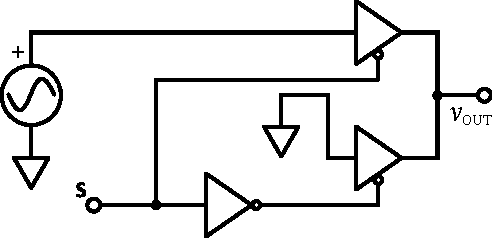
\includegraphics[width=.4\textwidth]{../E10/latex/impedence.pdf}
\caption{Circuito per trasmissione \textit{half duplex} costruito mediante l'utilizzo di porte 3State. Esso permette di condividere lo stesso canale trasmissivo.}
\label{cir10:3state}
\end{wrapfigure}

In questa parte abbiamo realizzato un circuito per trasmissione half-duplex tramite porte 3State.
Il fine di tale operazione è quello di condividere lo stesso canale per la trasmissione dei dati.
Possiamo dunque, semplicemente cambiando il segnale di controllo, decidere quale segnale deve essere trasmesso.
Ciò, come si vedrà nella seguente sezione, è particolarmente utile nel caso in cui si abbiano molti segnali da trasmettere.
Il circuito da noi implementato è quello riportato in figura.
Ricordiamo che le porte 3State da noi utilizzate sono attivate se il controllo è a 0 logico mentre sono ad "alta impedenza" se il controllo è ad 1 logico.
Dunque il circuito da noi costruito permetterà di selezionare uno dei due segnali e, sfruttando lo stato "alta impedenza", evitiamo cortocircuiti tra le uscite.

Il circuito è stato testato utilizzando la schedina a led.
